\chapter{System Perspective}

\section{System Design}

The present \texttt{MiniTwit} system represents a refactored and optimized version of the legacy \textit{Python} codebase that was originally provided. The present system is organized into three distinct components\footnote{To ensure consistency, programming languages, frameworks, and libraries will be presented in \textit{italics}.}, including i) a \textit{C\# ASP.NET} project that functions as the \textit{backend component}, ii) a \textit{React-based frontend component}, and iii) a \textit{NoSql MongoDB database}. These particular technologies were selected based on the developers existing familiarity with these tools, which has been achieved from prior courses and practical experience. 

\vspace{-0.2cm}
\begin{figure}[H]
    \centering
    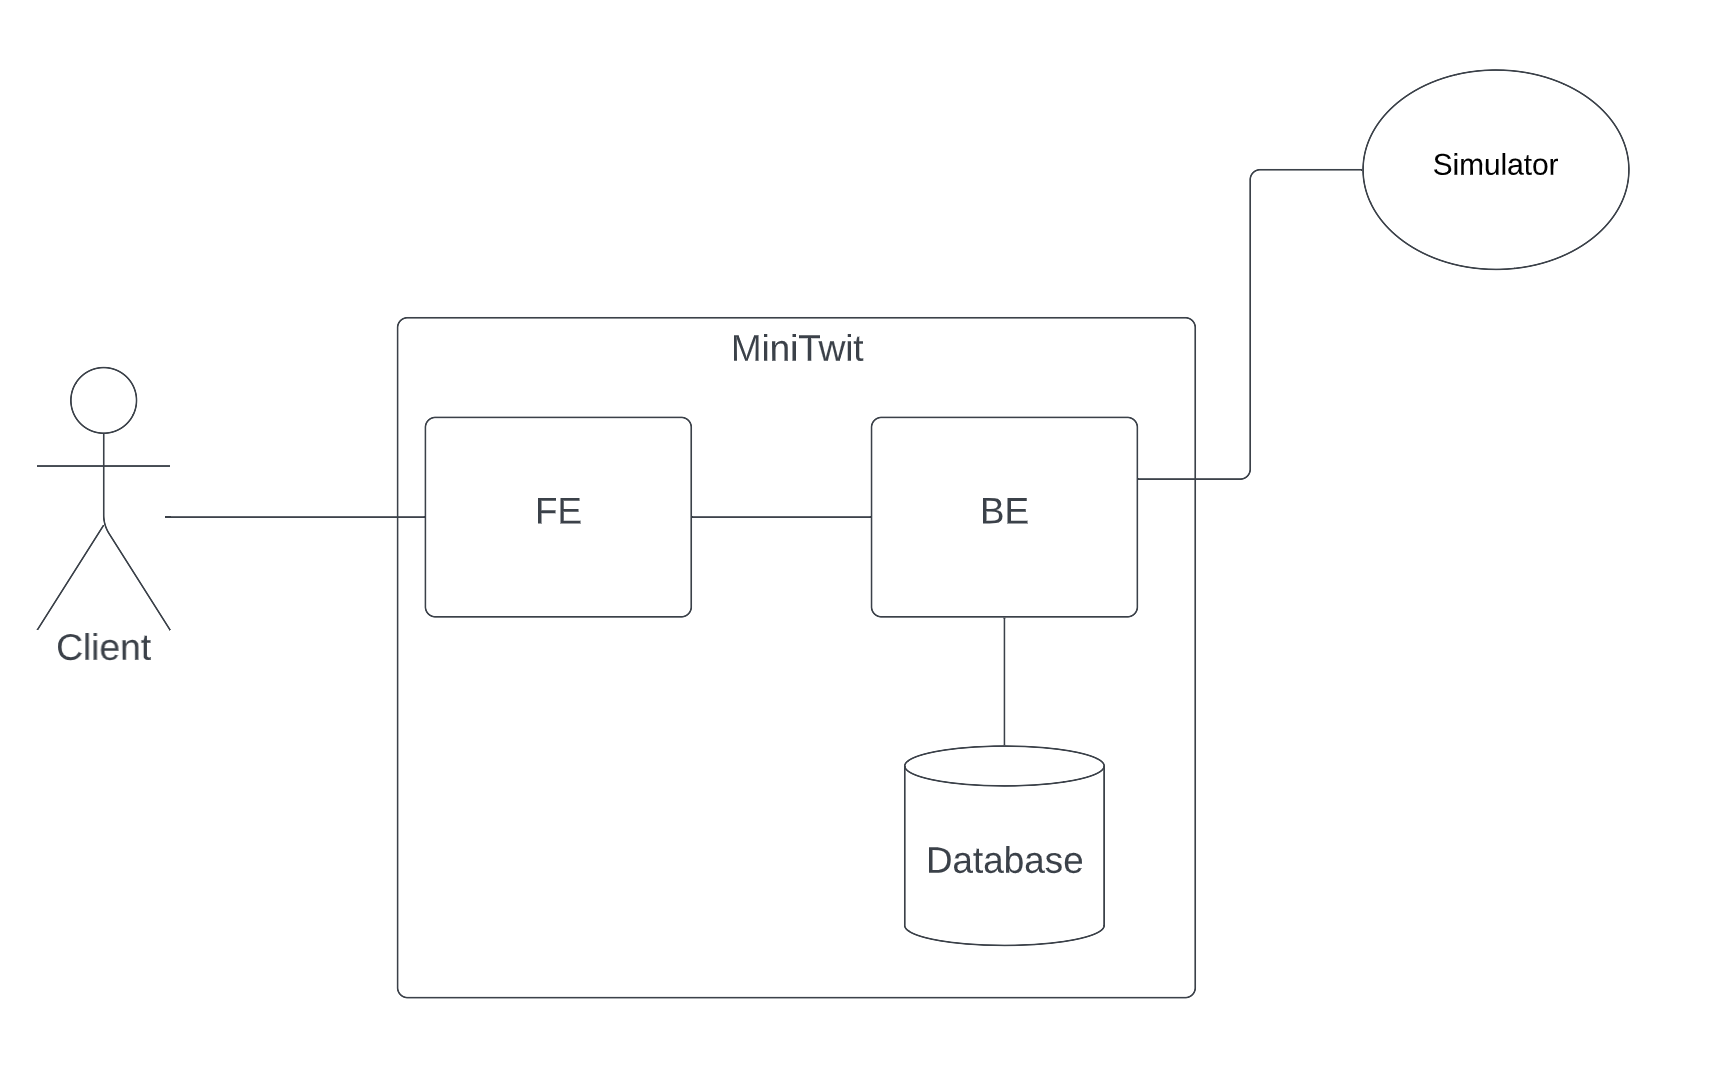
\includegraphics[width=12cm]{Use_case.png}
    \vspace{-0.6cm}
    \caption{System Design (use case)}
    \label{fig:use_case_diagram}
\end{figure}
\vspace{-0.4cm}

We quickly decided to create all services as Docker images, to avoid having separate local build scripts as we develop on different operating systems.

\subsection{System Architecture}

As shown in Figure \ref{fig:deployment_diagram}, \texttt{MiniTwit} is comprised of several subsystems. However, the two main components of the system are the \texttt{MiniTwit} frontend and backend. While further developing the components, we followed certain architectural patterns to ensure low coupling, high cohesion, and testability.

\begin{figure}[H]
    \centering
    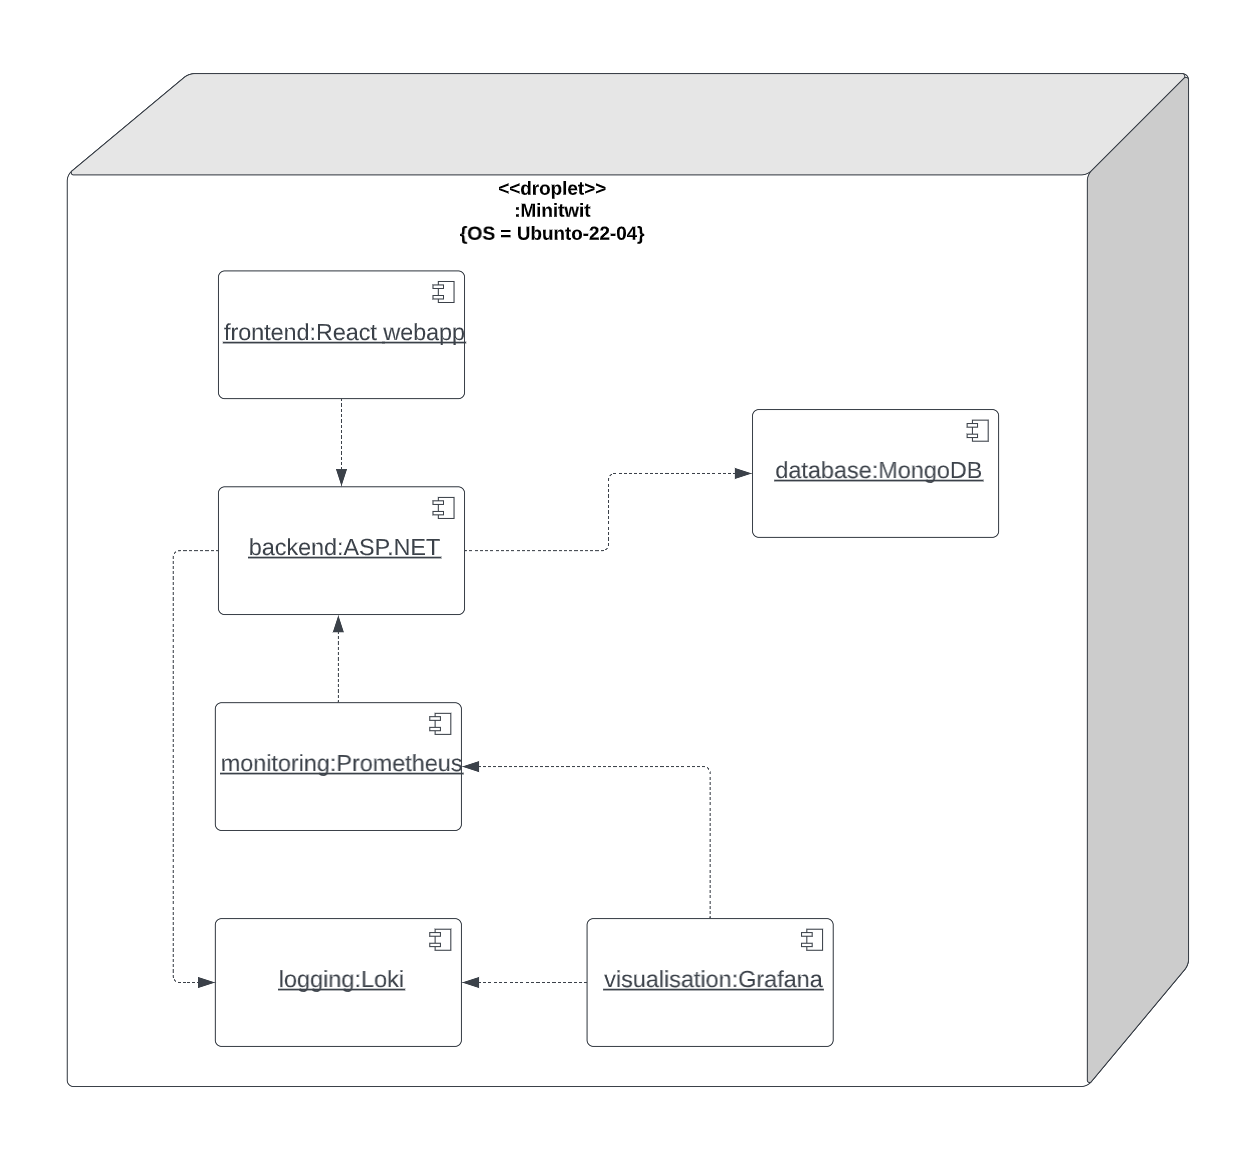
\includegraphics[width=14cm]{deployment_diagram.png}
    \vspace{-0.8cm}
    \caption{\texttt{Minitwit} deployment diagram.}
    \label{fig:deployment_diagram}
\end{figure}
\vspace{-0.3cm}

\subsubsection{MiniTwit Backend}
\label{sec:minitwit-backend-architecture}

The design of the \texttt{MiniTwit} backend is inspired by the \textit{Onion Architecture} (see Figure \ref{fig:backend-onion}) which is based on the \textit{Inversion of Control} principle. The architecture is comprised of multiple concentric layers that interface with each other toward the core. The flow of dependency goes inwards s.t. a layer only depends on the layers that come before it. Keeping the layers separate, makes them easier to test and maintain, as the coupling between them is kept low \cite{onion-architecture}.

\begin{figure}[H]
    \centering
    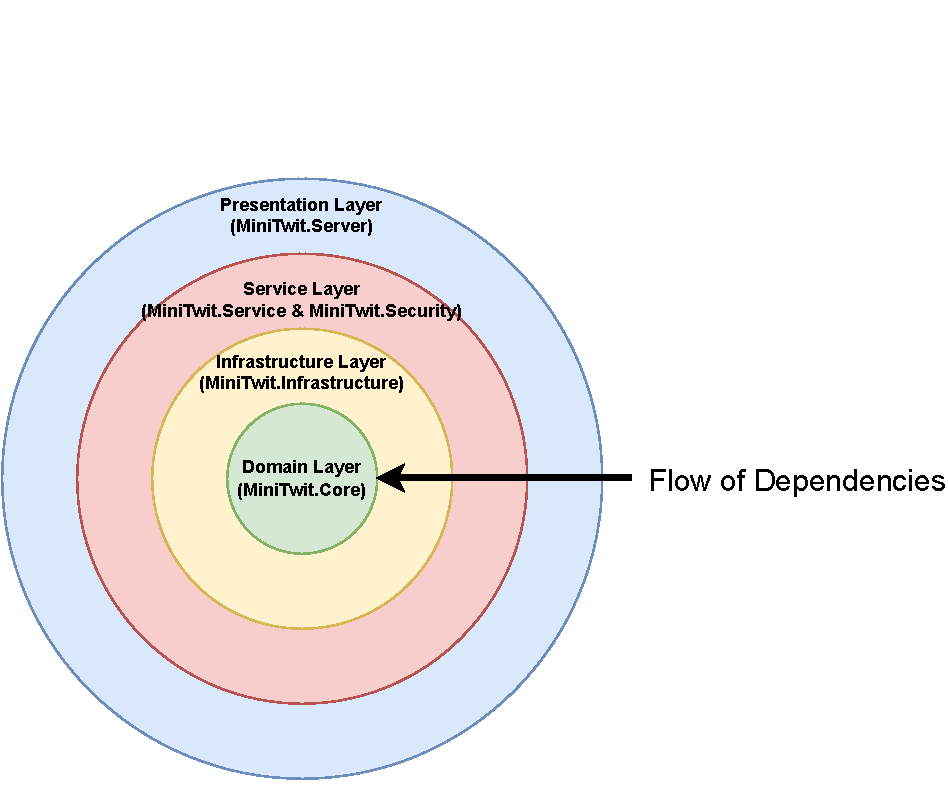
\includegraphics[scale=0.8]{architecture/onion.pdf}
    \caption{The Onion Architecture-based architecture of the \texttt{MiniTwit} backend.}
    \label{fig:backend-onion}
\end{figure}
\vspace{-0.3cm}

We chose to split the backend into four layers and five separate C\# projects (see figure \ref{fig:backend-onion}):

\begin{enumerate}
    \item \textbf{Domain Layer (MiniTwit.Core):} Contains the domain models, data transfer objects (\texttt{DTOs}), and interfaces for the business logic implemented in the next layer.
    \item \textbf{Infrastructure Layer (MiniTwit.Infrastructure):} Contains the business logic and database abstraction layer.
    \item \textbf{Service Layer (MiniTwit.Service \& MiniTwit.Security):} Is split in two projects; Service and Security:
    \begin{itemize}[$\circ$]
        \item \textbf{Service:} Contains abstractions to the infrastructure layer in the form of services.
        \item \textbf{Security:} Contains security-related abstractions in the form of hashing algorithms.
    \end{itemize}
    \item \textbf{Presentation Layer (MiniTwit.Server):} Contains the main API of the backend in the form of controllers and authentication schemes.
\end{enumerate}

As can be seen in the package diagram in Figure \ref{fig:backend-architecture}, the various layers only depend on the layers that come before them.

\begin{sidewaysfigure}[H]
    \centering
    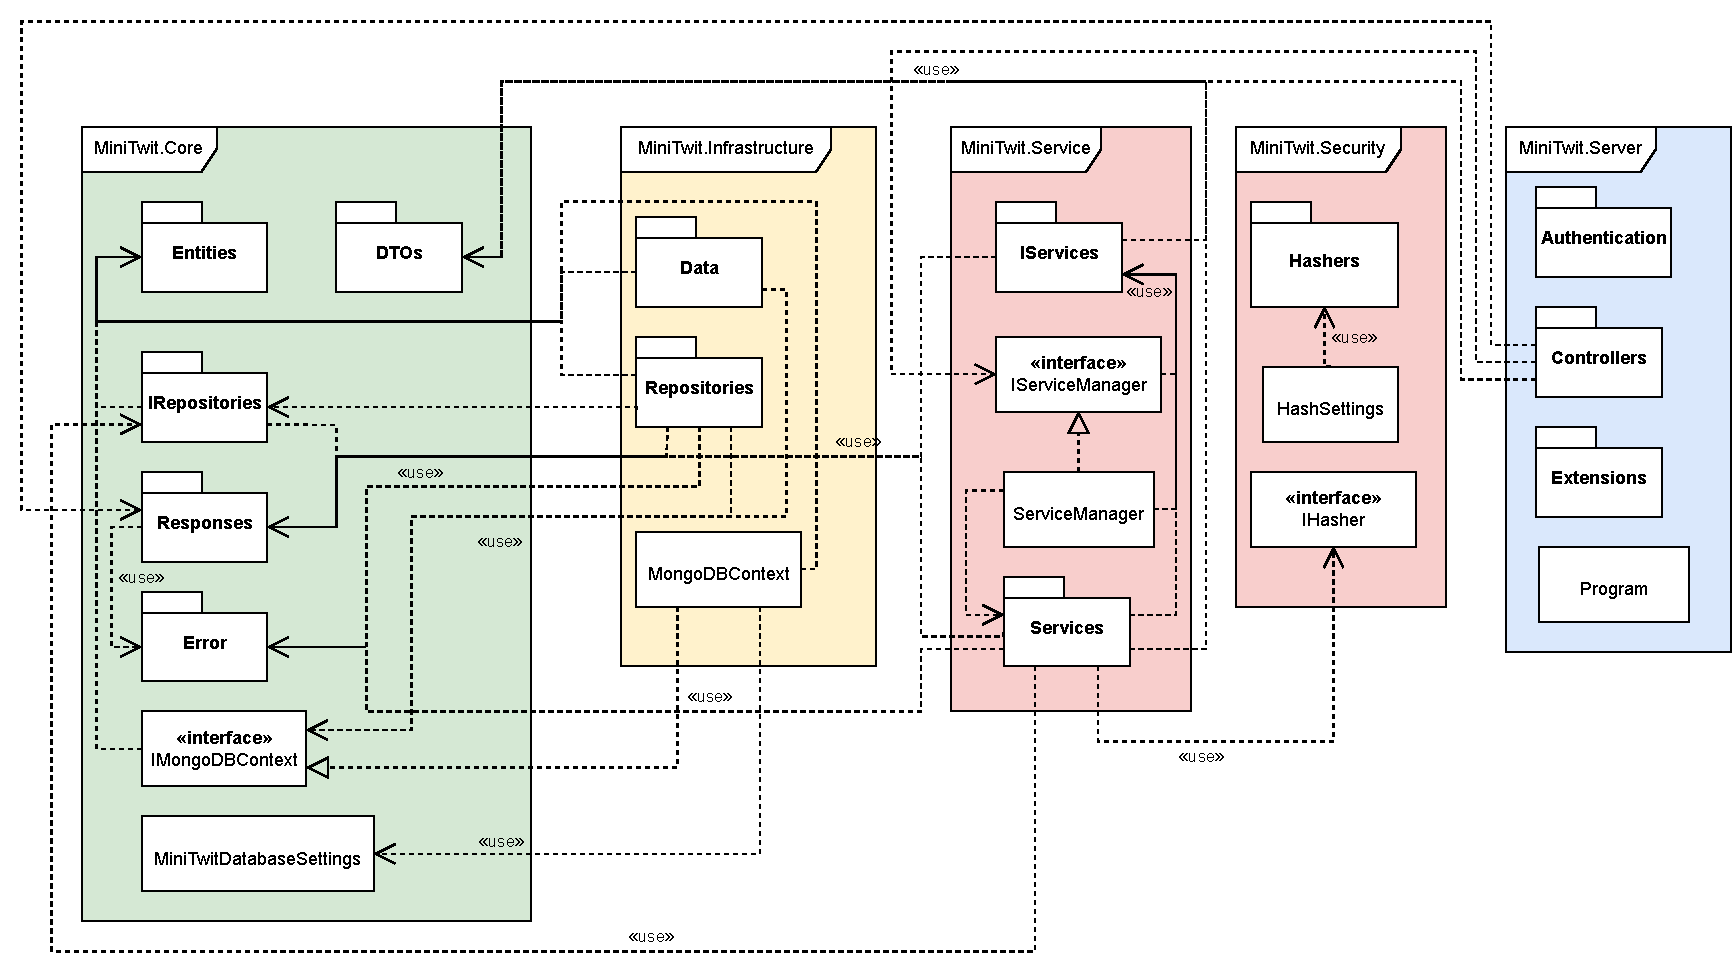
\includegraphics[width=\textwidth]{architecture/backend_package.pdf}
    \caption{Package diagram showing the contents of the various components of the \texttt{MiniTwit} backend.}
    \label{fig:backend-architecture}
\end{sidewaysfigure}

\subsubsection{MiniTwit Frontend}

The \texttt{MiniTwit} frontend, a \texttt{React} web app, was designed by splitting the functionalities of the web app into several packages to ensure maintainability and low coupling, and high cohesion. The packages include:

\begin{itemize}
    \item \textbf{models:} Contains the domain-specific interfaces provided by the backend API.
    \item \textbf{services:} Contains abstractions per domain-specific model used to communicate with the backend.
    \item \textbf{components:} Contains various web components used in the web pages of \texttt{MiniTwit}.
    \item \textbf{pages:} Contains all pages displayed on the \texttt{MiniTwit} website.
    \item \textbf{state:} Contains functions to update and read entries from the session storage of a client's web browser.
\end{itemize}

The various packages of the front end and their dependencies are shown in the expanded package diagram in figure \ref{fig:frontend-architecture}.

\begin{figure}[H]
    \centering
    \includegraphics[width=10cm]{example-image-a}
    \caption{The architecture of the \texttt{MiniTwit} frontend.}
    \label{fig:frontend-architecture}
\end{figure}

\section{System Dependencies}

By using \url{fossa.com} to analyze our project, we can conclude that our project contains 44 direct dependencies and 949 transitive dependencies. The dependencies are divided into \textit{NPM} dependencies for the frontend, \textit{C\#} application dependencies for the backend, and CI/CD dependencies in the form of GitHub Actions.  The \textit{NPM} dependencies are primarily \textit{React} libraries and the backend dependencies are primarily \textit{Mongo} and \textit{Microsoft} dependencies. The CI/CD dependencies in the form of GitHub Actions are a mix of many dependencies. The major concern is the direct dependencies, as they are the ones directly targeted in our code. However, the transitive dependencies can also be an issue. 

The above-mentioned dependencies can be seen listed per subcomponent of \texttt{MiniTwit} in Appendix \ref{appendix:dependencies}.

\section{Current State}

To obtain a comprehensive understanding of the current state of our system, this section outlines the status of three static analysis tools: \textit{ESLint}, \textit{CodeQL}, and \textit{Snyk}. Additionally, we provide our quality assessments from \textit{SonarCloud} and \textit{Code Climate}. Finally, the system's quality is evaluated through unit-, integration-, and UI tests. These three quality gates test the software quality in different ways and serve as an important benchmark for evaluating the system's overall quality.

Both the Status Analysis Tools and the Quality Assessments form part of a \textit{product view}, where the focus is on internal software metrics. In contrast, UI tests are highly relevant to the \textit{user view} since they assess the frontend behavior, which is the only access level for the client/user \cite[pp. 13-15]{kitchenham1996software}.

\subsection{Static Analysis Tools}

\textit{ESList} (TypeScript), \textit{CodeQL} (C\#), and \textit{Snyk} (security) serve as benchmarks of quality for the various languages and tools in our repository. Changes to the code that fail the quality gate metrics on certain parameters must be addressed before they can proceed in the CI/CD chain. However, for code that passes the quality gates and only exhibits minor warnings, it may move forward. For a more detailed explanation of the various \texttt{YAML} scripts, refer to section \ref{sec:ci-cd}.

\subsection{Quality Assessments}

\textit{SonarCloud} and \textit{Code Climate} (see figure \ref{fig:sonarcloud} and \ref{fig:codeclimate}) automatically scan the entire code base and grade the quality. Furthermore, it highlights what can be improved to obtain higher marks.

\begin{figure}[H]
    \centering
    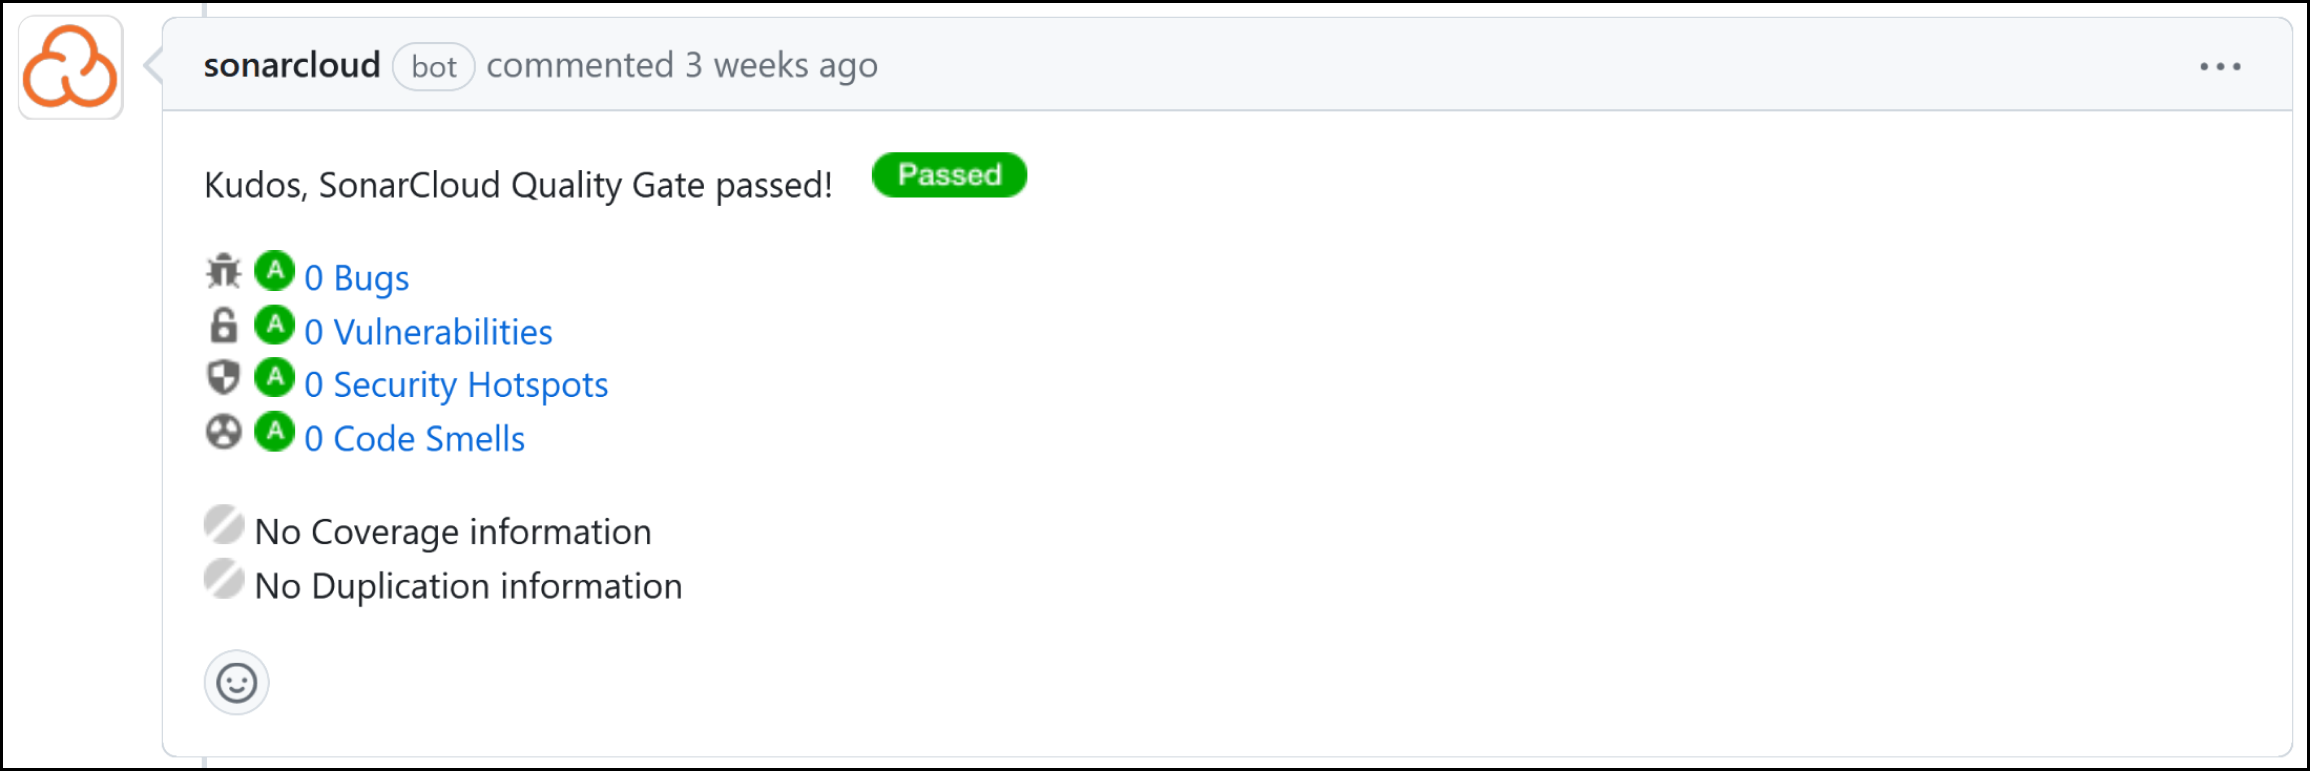
\includegraphics[width=12cm]{sonarcloud.png}
    \caption{\textit{SonarCloud} issue detector for pull request.}
    \label{fig:sonarcloud}
\end{figure}

\begin{figure}[H]
    \centering
    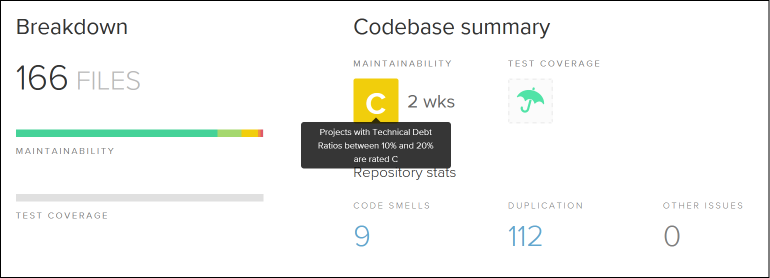
\includegraphics[width=12cm]{codeclimate.png}
    \caption{\textit{Code Climate} code base summary.}
    \label{fig:codeclimate}
\end{figure}

\subsection{Tests}

The back- and front-end testing are crucial quality checkpoints, as a failure in either would prevent the deployment of the system (see figure \ref{fig:tests}). Unit-, integration-, and UI tests have been implemented, but end-to-end tests have not been finalized. Testing of the backend's Onion Architecture, as described in section \ref{sec:minitwit-backend-architecture}, was done using 39 unit tests. Additionally, 17 integration tests were employed to test the behavior of the combined layers.

\begin{figure}[H]
    \centering
    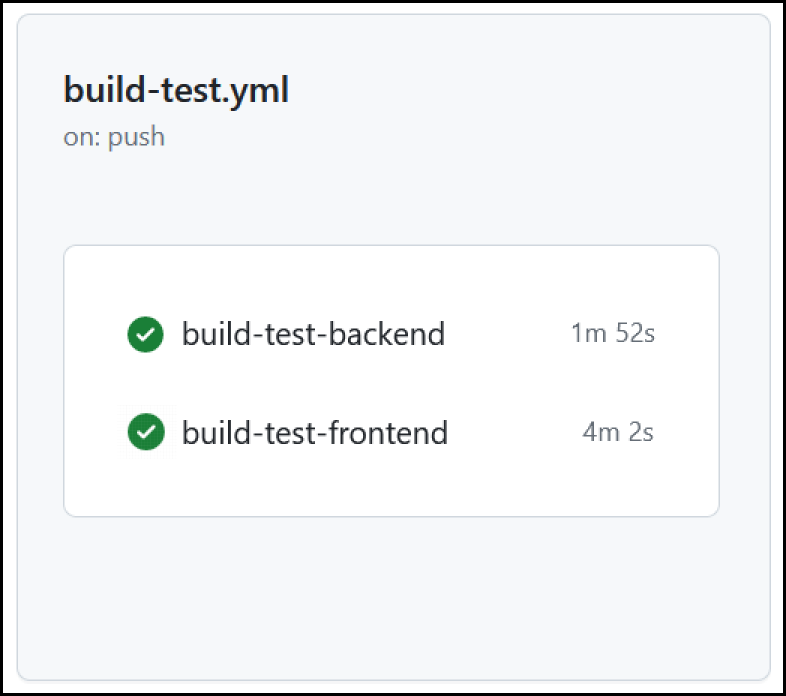
\includegraphics[width=5cm]{build-test.png}
    \caption{Chain of back- and frontend tests}
    \label{fig:tests}
\end{figure}

\section{Licence Compatability}

This project uses an \texttt{MIT} license. \texttt{MIT} is one of the most permissive licenses and therefore also compatible with other open source licenses \cite{wheeler:floss-license-slide}.  All licenses found in the direct dependencies can be seen in appendix \ref{appendix:dependencies}.